\documentclass{article}

%%%%%%%%%%%%%%% LIBRERIAS %%%%%%%%%%%%%%%%%%%%%
\usepackage[thinc]{esdiff}
\usepackage{amsmath,amssymb}
\usepackage{caption}
\usepackage{titlesec}
\usepackage{titletoc}
\usepackage{graphicx}
\IfFileExists{spanish.ldf}
  {\usepackage[spanish,es-tabla]{babel}}
  {\usepackage[provide=*,spanish]{babel}}
\usepackage{icomma}
\usepackage{xurl}
\usepackage{hyperref}
\usepackage{float}
\usepackage[table]{xcolor}
\usepackage{circuitikz}
\usepackage[left=2cm, right=2cm, top=2cm, bottom=2cm, footskip=1cm]{geometry}
\usepackage{subcaption}
\usepackage{booktabs}
\usepackage{array}
\usepackage{longtable}
\usepackage{tabularx}
\usepackage{enumitem}
\usepackage{setspace}
\usepackage{fancyhdr}
\usetikzlibrary{babel,arrows.meta,calc,positioning,decorations.pathmorphing}

%%%%%%%%%%%%%%%%%%% VARIABLES %%%%%%%%%%%%%%%%%%%%
\newcommand{\Facultad}{Instituto Tecnológico \\de\\ Buenos Aires}
\newcommand{\TPn}{Trabajo Práctico N° 4}
\newcommand{\TPtema}{Medición de la constante de Planck con LED}
\graphicspath{{figuras/}}

%%%%%%%%%%%%%%%%%% FORMATO TÍTULO Y NUMERACIÓN %%%%%%%%%%%%%%%%%%%
\renewcommand{\thesection}{\arabic{section}.}
\renewcommand{\thesubsection}{\thesection\arabic{subsection}}
\setcounter{secnumdepth}{3}

\titleformat{\section}{\Large\bfseries}{\thesection}{1em}{}
\titleformat{\subsection}{\large\bfseries}{\thesubsection}{0.5em}{}
\titleformat{\subsubsection}{\normalsize\bfseries}{\thesubsubsection}{0.5em}{}

%%%%%%%%%%%%%%% SOPORTE DEL CUERPO DEL INFORME %%%%%%%%%%%%%%%%%%%%%
\definecolor{azulencabezado}{HTML}{163A5F}
\definecolor{ledrojo}{HTML}{C0392B}
\definecolor{ledamarillo}{HTML}{B8760B}
\definecolor{ledverde}{HTML}{1E8449}
\definecolor{ledazul}{HTML}{2167AC}
\newcolumntype{Y}{>{\raggedright\arraybackslash}X}
\newcolumntype{C}[1]{>{\centering\arraybackslash}p{#1}}
\newcolumntype{L}[1]{>{\raggedright\arraybackslash}p{#1}}
\newcommand{\Js}{\ \mathrm{J\,s}}

\hypersetup{
  hidelinks,
  pdftitle={Informe del experimento de Medición de la constante de Planck con LED},
  pdfsubject={Laboratorio de Física IV},
  pdfkeywords={Constante de Planck, LED, semiconductores, laboratorio, Física IV}
}

\makeatletter
\providecommand{\ttl@finishall}{}
\makeatother

%%%%%%%%%%%%%%%%%%% ARCHIVO %%%%%%%%%%%%%%%%%%%%%%%%
\begin{document}
\renewcommand{\tablename}{Tabla}
\hypersetup{pageanchor=false}

%%%CARATULA%%%
\begin{titlepage}

        \begin{flushleft}
            \centering
            
\includegraphics[width=0.3\textwidth]{Logo_ITBA.png}
        \end{flushleft}

        \centering

        {\scshape\LARGE \Facultad\par}
        \vspace{1cm}

        {\huge\bfseries \TPn\par}
        \vspace{1.5cm}
        {\Large Laboratorio de Física IV\\ 93.61 \par}
        \vspace{0.5cm}
        {\Large \TPtema\par}
        \vspace{0.5cm}
        {\large Docente a cargo: Raúl Florentino\par}
        \vfill
        {\Large \bfseries Grupo N° 55 \par}
        \vspace{1cm}
        {\large Juan Ignacio Fogolin Lagares \hfill Legajo: 66409  \par}
        {\large Rita Moschini \hfill Legajo: 67026 \par}
        {\large Agustín Alejandro Montoto \hfill Legajo: 65511\par}
        \vfill
        {\large Fecha de entrega: \today\par}
        \vfill

        \begin{flushleft}
        \renewcommand{\arraystretch}{2.2}
        \begin{tabularx}{\textwidth}{@{}L{8.5cm}Y@{}}
            \toprule
            \textbf{Fecha de aprobación:} & \\
            \midrule
            \textbf{Comentarios y observaciones del docente:} & \\
             & \\
             & \\
            \bottomrule
        \end{tabularx}
        \end{flushleft}

\end{titlepage}

\pagenumbering{gobble}
\tableofcontents
\newpage

%%%%%%%%%%%%%%%%%%% CUERPO DEL INFORME %%%%%%%%%%%%%%%%%%%%%%%%
\pagenumbering{arabic}
\setcounter{page}{1}
\hypersetup{pageanchor=true}

\setstretch{1.12}
\setlength{\parindent}{0.7cm}
\setlength{\parskip}{0.25em}
\setlength{\arrayrulewidth}{0.45pt}
\setlength{\tabcolsep}{5pt}
\arrayrulecolor{black}
\renewcommand{\arraystretch}{1.22}

\renewcommand{\thesection}{\arabic{section}}
\renewcommand{\thesubsection}{\thesection.\arabic{subsection}}
\renewcommand{\thesubsubsection}{\thesubsection.\arabic{subsubsection}}
\setcounter{secnumdepth}{3}

\titleformat{\section}{\Large\bfseries\color{black}}{\thesection}{0.6em}{}
\titleformat{\subsection}{\large\bfseries\color{black}}{\thesubsection}{0.55em}{}
\titlespacing*{\section}{0pt}{1.1em}{0.45em}
\titlespacing*{\subsection}{0pt}{0.9em}{0.35em}

\captionsetup{font={small,it},labelfont=it,justification=centering}
\setlist[itemize]{leftmargin=1.05cm,itemsep=0.18em,topsep=0.25em}
\setlist[enumerate]{leftmargin=1.05cm,itemsep=0.22em,topsep=0.25em}

\pagestyle{fancy}
\fancyhf{}
\fancyhead[L]{\small\itshape{} Laboratorio de Física IV\/}
\fancyhead[R]{\small\itshape{} Instituto Tecnológico de Buenos Aires\/}
\fancyfoot[C]{\thepage}
\renewcommand{\headrulewidth}{0pt}
\renewcommand{\footrulewidth}{0pt}

%=====================================================================
\section{Objetivos y resumen}

\subsection{Objetivos}

\begin{itemize}
    \item Determinar experimentalmente la constante de Planck $h$ a partir de la relación $E=h\nu$, aplicada a la luz emitida por cuatro diodos emisores de luz (LED) de distinto color.
    \item Obtener la tensión umbral $V_g$ de cada LED a partir de su curva característica $I(V)$, mediante la extrapolación de la zona lineal hasta corriente nula (método de O'Connor), y medir con un espectrómetro la longitud de onda de su pico de emisión.
    \item Calcular el error porcentual de cada determinación respecto del valor de referencia, estimar las incertidumbres e interpretar físicamente las discrepancias observadas.
\end{itemize}

\subsection{Resumen}

En un LED, cada electrón que atraviesa la juntura p-n y se recombina con un hueco puede emitir un fotón cuya energía es aproximadamente igual al ancho de la banda prohibida del semiconductor, $E_g$. Para que circule una corriente apreciable, la tensión aplicada debe compensar la barrera de potencial de la juntura, que es del orden de $E_g/e$. Igualando la energía que recibe cada electrón, $eV_g$, con la energía del fotón emitido, $hc/\lambda$, es posible despejar la constante de Planck.

Para cada uno de los cuatro LEDs (rojo, amarillo, verde y azul) se midió la longitud de onda del pico de emisión con un espectrómetro y se registraron 15 pares de valores de tensión y corriente, desde el inicio de la conducción hasta unos $30\ \mathrm{mA}$. La zona lineal de cada curva ($I\geq10\ \mathrm{mA}$) se ajustó por mínimos cuadrados y se extrapoló hasta $I=0$ para obtener $V_g$. Con estos valores se calculó $h_e=eV_g\lambda/c$ para cada LED, junto con su incertidumbre y su error porcentual.

\textbf{Resultados principales:} los LEDs rojo y amarillo dieron $h_e=(6,02\pm0,05)\times10^{-34}\Js$ y $(5,97\pm0,04)\times10^{-34}\Js$, un $9\%$ y un $10\%$ por debajo del valor de referencia. Los LEDs verde y azul dieron $(7,84\pm0,05)\times10^{-34}\Js$ y $(7,15\pm0,07)\times10^{-34}\Js$, un $18\%$ y un $8\%$ por encima. El promedio de los cuatro valores, $\overline{h}_e=(6,7\pm0,5)\times10^{-34}\Js$, difiere en un $1,9\%$ del valor de referencia, aunque este buen acuerdo resulta de la compensación entre desvíos sistemáticos de signo opuesto, que se asocian a los distintos materiales semiconductores de los LEDs.

%=====================================================================
\section{Introducción teórica}

\subsection{Cuantización de la energía de la radiación}

En 1900, para explicar el espectro de la radiación del cuerpo negro, Max Planck postuló que la energía de un oscilador de frecuencia $\nu$ solo puede intercambiarse en cantidades discretas, múltiplos de $h\nu$. En 1905 Einstein extendió la idea a la propia radiación, que está formada por cuantos de luz (fotones) de energía
\begin{equation}
    E=h\nu=\frac{hc}{\lambda},
    \label{eq:foton}
\end{equation}
donde $h$ es la constante de Planck, $c$ la velocidad de la luz y $\lambda$ la longitud de onda \cite{eisberg}. Desde 2019 el valor de $h$ es exacto por definición del Sistema Internacional: $h=6,62607015\times10^{-34}\Js$ \cite{codata}. En este trabajo, siguiendo la consigna \cite{consigna}, se toma como referencia $h_{\mathrm{teo}}=6,62\times10^{-34}\Js$, con $c=2,99\times10^{8}\ \mathrm{m/s}$ y $e=1,602\times10^{-19}\ \mathrm{C}$.

\subsection{Semiconductores y juntura p-n}

En un sólido cristalino los niveles de energía de los electrones se agrupan en bandas. En un semiconductor, la última banda llena (banda de valencia, de borde superior $E_V$) está separada de la siguiente (banda de conducción, de borde inferior $E_C$) por una banda prohibida de ancho $E_g=E_C-E_V$, del orden de 1 a 3~eV. Al dopar el material con impurezas se obtiene un semiconductor tipo n (exceso de electrones en la banda de conducción) o tipo p (exceso de huecos en la banda de valencia).

Al unir ambos tipos se forma una juntura p-n. Los portadores difunden a través de la unión y dejan una zona de carga espacial cuyo campo eléctrico genera una barrera de potencial de altura $eV_{bi}\lesssim E_g$, que impide que siga circulando corriente. Al aplicar una polarización directa $V$, la barrera se reduce a $e(V_{bi}-V)$: los electrones del lado n y los huecos del lado p se inyectan en la región de la juntura y allí se recombinan (Figura~\ref{fig:bandas}).

\begin{figure}[H]
\centering
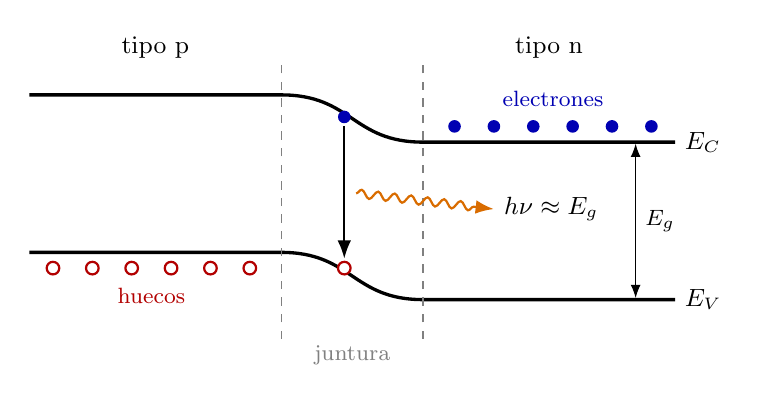
\begin{tikzpicture}[x=1cm,y=1cm,>=Latex,font=\small]
    % bandas en polarización directa
    \draw[very thick] (0,2.7) -- (3.2,2.7) .. controls (4.1,2.7) and (4.1,2.1) .. (5.0,2.1) -- (8.2,2.1);
    \draw[very thick] (0,0.7) -- (3.2,0.7) .. controls (4.1,0.7) and (4.1,0.1) .. (5.0,0.1) -- (8.2,0.1);
    \node[right] at (8.2,2.1) {$E_C$};
    \node[right] at (8.2,0.1) {$E_V$};
    \node at (1.6,3.3) {tipo p};
    \node at (6.6,3.3) {tipo n};
    \draw[dashed,gray] (3.2,-0.4) -- (3.2,3.1);
    \draw[dashed,gray] (5.0,-0.4) -- (5.0,3.1);
    \node[gray,font=\footnotesize] at (4.1,-0.6) {juntura};
    % electrones y huecos
    \foreach \x in {5.4,5.9,6.4,6.9,7.4,7.9} \fill[blue!70!black] (\x,2.3) circle (0.08);
    \foreach \x in {0.3,0.8,1.3,1.8,2.3,2.8} \draw[red!70!black,thick,fill=white] (\x,0.5) circle (0.08);
    \node[blue!70!black,font=\footnotesize] at (6.65,2.65) {electrones};
    \node[red!70!black,font=\footnotesize] at (1.55,0.15) {huecos};
    % recombinación
    \fill[blue!70!black] (4.0,2.42) circle (0.08);
    \draw[->,thick] (4.0,2.3) -- (4.0,0.62);
    \draw[red!70!black,thick,fill=white] (4.0,0.5) circle (0.08);
    \draw[->,decorate,decoration={snake,amplitude=1.5pt,segment length=6pt,post length=2mm},orange!85!black,thick] (4.15,1.45) -- (5.9,1.25) node[right,black] {$h\nu\approx E_g$};
    % Eg
    \draw[<->] (7.7,0.12) -- node[right,font=\footnotesize] {$E_g$} (7.7,2.08);
\end{tikzpicture}
\caption{Diagrama de bandas simplificado de una juntura p-n en polarización directa: los electrones y huecos inyectados se recombinan en la juntura y emiten fotones de energía $h\nu\approx E_g$.}
\label{fig:bandas}
\end{figure}

\subsection{Emisión de luz en un LED}

En los semiconductores de banda prohibida directa, la recombinación de un electrón con un hueco es mayoritariamente radiativa: la energía liberada se emite como un fotón. Como los portadores ocupan estados cercanos a los bordes de las bandas, con una dispersión térmica del orden de $k_BT$, la luz emitida es casi monocromática y su energía de pico vale aproximadamente \cite{schubert}
\begin{equation}
    h\nu_{\mathrm{pico}}\approx E_g+\tfrac{1}{2}k_BT,
    \label{eq:pico}
\end{equation}
con un ancho espectral de unos $1,8\,k_BT\approx46\ \mathrm{meV}$ a temperatura ambiente. El color de un LED queda así determinado por el material: los LEDs rojos, naranjas y amarillos suelen fabricarse con AlGaInP, y los verdes, azules y violetas con InGaN, ajustando la composición de la aleación para obtener el $E_g$ deseado \cite{schubert}. Como $k_BT\approx26\ \mathrm{meV}$ es mucho menor que $E_g$, puede tomarse $E_g\approx hc/\lambda_{\mathrm{pico}}$.

\subsection{Característica corriente-tensión y tensión umbral}

La corriente en una juntura ideal sigue la ecuación de Shockley,
\begin{equation}
    I=I_s\left[\exp\left(\frac{eV_j}{\eta\,k_BT}\right)-1\right],
    \label{eq:shockley}
\end{equation}
donde $V_j$ es la tensión sobre la juntura, $\eta$ el factor de idealidad (entre 1 y 2) e $I_s$ la corriente de saturación, que es proporcional a $\exp(-E_g/\eta k_BT)$ y resulta extremadamente pequeña. Por esta razón la corriente es prácticamente nula mientras $eV_j$ es bastante menor que $E_g$, y crece de forma abrupta cuando la tensión se acerca a $E_g/e$, es decir, cuando la barrera de la juntura prácticamente desaparece \cite{sze}.

En un dispositivo real existe además una resistencia en serie $R_s$ (contactos y regiones neutras), de modo que la tensión en bornes es $V=V_j+IR_s$. A corrientes altas la juntura ya está ``abierta'' y casi todo aumento de tensión cae sobre $R_s$, por lo que la curva $I(V)$ se vuelve aproximadamente lineal. Siguiendo a O'Connor y O'Connor \cite{oconnor}, se define la \textbf{tensión umbral} $V_g$ como la intersección de la prolongación de esa recta con el eje de tensiones ($I=0$), y se la identifica con la energía de la banda prohibida:
\begin{equation}
    E_g=e\,V_g.
    \label{eq:Vg}
\end{equation}

\subsection{Determinación de la constante de Planck}

Igualando la energía \eqref{eq:Vg} que adquiere cada portador con la energía \eqref{eq:foton} del fotón emitido se obtiene
\begin{equation}
    e\,V_g=\frac{h\,c}{\lambda}
    \qquad\Longrightarrow\qquad
    h_e=\frac{e\,V_g\,\lambda}{c},
    \label{eq:he}
\end{equation}
donde $h_e$ es el valor experimental de la constante de Planck. Su error porcentual respecto del valor de referencia es
\begin{equation}
    \mathrm{Error}\%=\frac{\left|h_{\mathrm{teo}}-h_e\right|}{h_{\mathrm{teo}}}\times100\%.
    \label{eq:error}
\end{equation}

%=====================================================================
\section{Instrumentos y elementos empleados}

\begin{longtable}{@{}L{4.0cm}L{6.8cm}L{5.4cm}@{}}
    \caption{Instrumentos y elementos del montaje experimental.}\label{tab:instrumentos}\\
    \toprule
    \textbf{Elemento} & \textbf{Función} & \textbf{Especificación relevante} \\
    \midrule
    \endfirsthead
    \toprule
    \textbf{Elemento} & \textbf{Función} & \textbf{Especificación relevante} \\
    \midrule
    \endhead
    \bottomrule
    \endfoot
    Dispositivo con LEDs & Contiene los cuatro LEDs y un regulador que permite variar la corriente que circula por cada uno. & LEDs rojo, amarillo, verde y azul; $I_{\max}\approx30\ \mathrm{mA}$ \\
    Fuente de tensión continua & Alimenta el dispositivo. & $5\ \mathrm{V}$ \\
    Amperímetro & Mide la corriente $I$ que circula por el LED. & Escala de mA \\
    Voltímetro & Mide la tensión $V$ en bornes del LED. & Escala de $20\ \mathrm{V}$; resolución $0,01\ \mathrm{V}$ \\
    Fibra óptica & Conduce la luz del LED hasta el espectrómetro. & Se desconecta por encima de $\approx4000$ cuentas \\
    Espectrómetro (espectrofotómetro) & Mide el espectro de emisión del LED y su longitud de onda de pico. & Resolución $\approx2\ \mathrm{nm}$ \\
    PC con SpectraSuite & Adquisición y visualización del espectro. & Lectura de $\lambda_{\mathrm{pico}}$ con cursor \\
\end{longtable}

\begin{figure}[H]
\centering
\begin{circuitikz}[american, line width=0.6pt, font=\small]
    \draw (0,0) to[battery1, l=$5\ \mathrm{V}$] (0,3)
          to[pR, l=$R_{\mathrm{reg}}$] (3,3)
          to[ammeter, l=$I$] (5.4,3) -- (7.6,3)
          to[full led, l_=LED] (7.6,0) -- (0,0);
    \draw (5.4,3) to[voltmeter, l_=$V$] (5.4,0);
    \draw[->,decorate,decoration={snake,amplitude=1.2pt,segment length=6pt,post length=2mm},orange!85!black,thick] (8.2,1.5) -- (10.4,1.5);
    \node[font=\footnotesize] at (9.3,1.9) {fibra óptica};
    \node[draw,rounded corners=2pt,minimum width=2.4cm,minimum height=1.1cm,align=center] (esp) at (11.7,1.5) {Espectrómetro};
    \node[draw,rounded corners=2pt,minimum width=2.4cm,minimum height=0.9cm,align=center] (pc) at (11.7,-0.3) {PC (SpectraSuite)};
    \draw[->] (esp.south) -- (pc.north);
\end{circuitikz}
\caption{Esquema eléctrico simplificado del montaje: el regulador del dispositivo fija la corriente por el LED, el amperímetro mide $I$ y el voltímetro la tensión $V$ en bornes del LED; la fibra óptica lleva la luz emitida al espectrómetro.}
\label{fig:circuito}
\end{figure}

%=====================================================================
\section{Procedimiento experimental}

Se siguió el procedimiento indicado en la guía de la cátedra \cite{consigna}:

\begin{enumerate}
    \item Se conectó el dispositivo a la fuente de $5\ \mathrm{V}$ y se conectaron el amperímetro (escala de mA) en serie y el voltímetro (escala de $20\ \mathrm{V}$) en paralelo con el LED.
    \item Se conectó la fibra óptica entre el dispositivo y el espectrómetro, y este a la PC con el programa SpectraSuite.
    \item Para cada LED se aumentó gradualmente la tensión desde cero y se registraron los pares $(V,I)$: primero algunos valores sin conducción y, a partir del umbral, valores crecientes de corriente hasta $30\ \mathrm{mA}$, con un total de 15 puntos por LED.
    \item Con la fibra conectada se leyó la longitud de onda del pico de emisión. Cuando la intensidad alcanzó unas 4000 cuentas se desconectó la fibra, para no saturar el espectrómetro, y se continuó con la medición eléctrica.
\end{enumerate}

%=====================================================================
\section{Datos obtenidos, discusión y cálculo de errores}

\subsection{Mediciones experimentales}

La Tabla~\ref{tab:datos} reúne las mediciones de la planilla. En el encabezado se indica la longitud de onda del pico de emisión de cada LED.

\begin{table}[H]
\centering\small
\caption{Tensión y corriente medidas para cada LED.}
\label{tab:datos}
\begin{tabular}{@{}c|cc|cc|cc|cc@{}}
\toprule
 & \multicolumn{2}{c|}{\textbf{Rojo} ($\lambda=628$ nm)} & \multicolumn{2}{c|}{\textbf{Amarillo} ($\lambda=595$ nm)} & \multicolumn{2}{c|}{\textbf{Verde} ($\lambda=530$ nm)} & \multicolumn{2}{c}{\textbf{Azul} ($\lambda=459$ nm)}\\
\textbf{Medición} & $V$ (V) & $I$ (mA) & $V$ (V) & $I$ (mA) & $V$ (V) & $I$ (mA) & $V$ (V) & $I$ (mA)\\
\midrule
1  & 0,00 & 0   & 0,00 & 0   & 0,00 & 0    & 0,00 & 0\\
2  & 0,50 & 0   & 0,50 & 0   & 0,50 & 0    & 0,50 & 0\\
3  & 1,00 & 0   & 1,00 & 0   & 1,00 & 0    & 1,00 & 0\\
4  & 1,50 & 0   & 1,50 & 0   & 1,50 & 0    & 1,50 & 0\\
5  & 1,67 & 0,1 & 1,73 & 0,1 & 2,40 & 0,1  & 2,58 & 0,1\\
6  & 1,72 & 1   & 1,80 & 1   & 2,62 & 1    & 2,72 & 1\\
7  & 1,75 & 2   & 1,82 & 2   & 2,68 & 2    & 2,79 & 2\\
8  & 1,78 & 4   & 1,85 & 4   & 2,76 & 4    & 2,88 & 4\\
9  & 1,80 & 6   & 1,87 & 6   & 2,81 & 6    & 2,95 & 6\\
10 & 1,83 & 8   & 1,88 & 8   & 2,86 & 8    & 3,00 & 8\\
11 & 1,84 & 10  & 1,90 & 10  & 2,89 & 10   & 3,04 & 10\\
12 & 1,88 & 15  & 1,92 & 15  & 2,97 & 15   & 3,14 & 15\\
13 & 1,91 & 20  & 1,93 & 20  & 3,04 & 20   & 3,22 & 20\\
14 & 1,93 & 25  & 1,95 & 25  & 3,10 & 25   & 3,28 & 25\\
15 & 1,96 & 30  & 1,96 & 30  & 3,16 & 29,6 & 3,34 & 30\\
\bottomrule
\end{tabular}
\end{table}

En todos los casos la corriente es nula hasta $1,5\ \mathrm{V}$ y aparece de forma abrupta a partir de cierta tensión, que es claramente mayor para los LEDs verde y azul (de menor $\lambda$, es decir, de mayor energía de fotón) que para el rojo y el amarillo. Este es el comportamiento cualitativo que predice la ecuación \eqref{eq:he}.

\subsection{Determinación de la tensión umbral \texorpdfstring{$V_g$}{Vg}}

De acuerdo con la consigna, se descartaron los valores de corriente menores a $1\ \mathrm{mA}$. Para definir la zona lineal se adoptó el mismo criterio objetivo para los cuatro LEDs: los cinco puntos de mayor corriente, $I\geq10\ \mathrm{mA}$. Por debajo de ese valor la curva todavía conserva la curvatura exponencial de la ecuación \eqref{eq:shockley}, como se observa en la Figura~\ref{fig:IV}.

Como la corriente fue la variable fijada (con valores redondos) y la tensión la variable leída, cada recta se ajustó por mínimos cuadrados en la forma
\begin{equation}
    V=V_g+r_d\,I,
    \label{eq:ajuste}
\end{equation}
cuya ordenada al origen es directamente la intersección de la recta con el eje de tensiones ($I=0$), y cuya pendiente $r_d$ es la resistencia dinámica del LED en la zona lineal. Esta recta es la misma tangente que se obtendría con la línea de tendencia $I(V)$ en Excel: ambos procedimientos dan valores de $V_g$ que difieren en menos de $0,005\ \mathrm{V}$.

\begin{figure}[H]
\centering
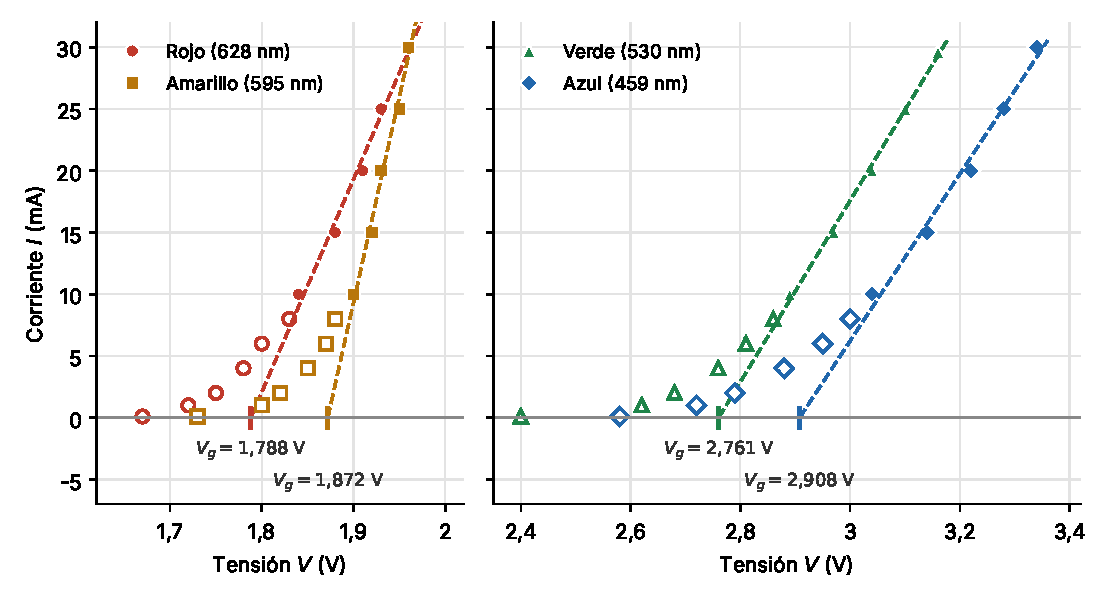
\includegraphics[width=\textwidth]{curvas_IV.pdf}
\caption{Curvas $I(V)$ de los cuatro LEDs. Los símbolos llenos son los puntos de la zona lineal utilizados en el ajuste ($I\geq10\ \mathrm{mA}$) y los huecos, los restantes puntos con $I>0$. Las rectas discontinuas son los ajustes extrapolados hasta $I=0$, donde se indica la tensión umbral $V_g$.}
\label{fig:IV}
\end{figure}

\begin{table}[H]
\centering\small
\caption{Resultados del ajuste lineal de la zona $I\geq10\ \mathrm{mA}$ (5 puntos por LED).}
\label{tab:ajuste}
\begin{tabular}{@{}lccccc@{}}
\toprule
\textbf{LED} & $\boldsymbol{\lambda}$ \textbf{(pico)} & $\boldsymbol{V_g}$ \textbf{(V)} & $\boldsymbol{r_d}$ \textbf{($\Omega$)} & $\boldsymbol{R^2}$\\
\midrule
\textcolor{ledrojo}{$\bullet$} Rojo         & 628 nm & $1,788\pm0,013$ & 5,8  & 0,987\\
\textcolor{ledamarillo}{$\bullet$} Amarillo & 595 nm & $1,872\pm0,011$ & 3,0  & 0,987\\
\textcolor{ledverde}{$\bullet$} Verde       & 530 nm & $2,761\pm0,014$ & 13,6 & 0,997\\
\textcolor{ledazul}{$\bullet$} Azul         & 459 nm & $2,908\pm0,024$ & 14,8 & 0,986\\
\bottomrule
\end{tabular}
\end{table}

\subsection{Cálculo de la constante de Planck}

Con la ecuación \eqref{eq:he} y las constantes de la consigna se obtiene $h_e$ para cada LED. Para el LED rojo, por ejemplo:

\begin{center}
\begin{tabular}{@{}ll@{}}
LED: & Rojo\\
$\lambda$ (pico): & $628\ \mathrm{nm}$\\
$V$ (gráfico): & $V_g=1,788\ \mathrm{V}$\\
\end{tabular}
\end{center}
\begin{equation*}
    h_e=\frac{e\,V_g\,\lambda}{c}=\frac{(1,602\times10^{-19}\ \mathrm{C})(1,788\ \mathrm{V})(628\times10^{-9}\ \mathrm{m})}{2,99\times10^{8}\ \mathrm{m/s}}=6,016\times10^{-34}\Js,
\end{equation*}
\begin{equation*}
    \mathrm{Error}\%=\frac{|6,62-6,016|}{6,62}\times100\%=9,1\%.
\end{equation*}

La Tabla~\ref{tab:planck} resume los resultados de los cuatro LEDs. La columna ``Desvío'' indica el signo de la diferencia: $h_e$ resulta menor que $h_{\mathrm{teo}}$ para los LEDs rojo y amarillo, y mayor para el verde y el azul.

\begin{table}[H]
\centering\small
\caption{Constante de Planck obtenida con cada LED y su error porcentual respecto de $h_{\mathrm{teo}}=6,62\times10^{-34}\ \mathrm{J\,s}$.}
\label{tab:planck}
\begin{tabular}{@{}lccccc@{}}
\toprule
\textbf{LED} & $\boldsymbol{\lambda}$ \textbf{(nm)} & $\boldsymbol{V_g}$ \textbf{(V)} & $\boldsymbol{h_e}$ \textbf{($\mathbf{10^{-34}}$ J\,s)} & \textbf{Error (\%)} & \textbf{Desvío}\\
\midrule
Rojo     & 628 & $1,788\pm0,013$ & $6,02\pm0,05$ & 9,1  & por defecto\\
Amarillo & 595 & $1,872\pm0,011$ & $5,97\pm0,04$ & 9,9  & por defecto\\
Verde    & 530 & $2,761\pm0,014$ & $7,84\pm0,05$ & 18,4 & por exceso\\
Azul     & 459 & $2,908\pm0,024$ & $7,15\pm0,07$ & 8,0  & por exceso\\
\midrule
\multicolumn{3}{@{}l}{Promedio de los cuatro LEDs} & $6,7\pm0,5$ & 1,9 & por exceso\\
\bottomrule
\end{tabular}
\end{table}

El promedio es $\overline{h}_e=6,744\times10^{-34}\Js$, y su incertidumbre se tomó como el error estándar de los cuatro valores, $s/\sqrt{4}=0,46\times10^{-34}\Js$, donde $s=0,91\times10^{-34}\Js$ es su desvío estándar.\footnote{Con los valores exactos del SI, $c=299\,792\,458\ \mathrm{m/s}$ y $e=1,602176634\times10^{-19}\ \mathrm{C}$, todos los $h_e$ disminuyen un $0,25\%$ y el promedio pasa a $6,73\times10^{-34}\Js$, un $1,5\%$ por encima de $h=6,62607\times10^{-34}\Js$. La elección de las constantes no altera, por lo tanto, las conclusiones.}

\subsection{Cálculo de errores}

\textbf{Incertidumbre de la tensión umbral.} La incertidumbre estadística de la ordenada al origen del ajuste \eqref{eq:ajuste} es
\begin{equation}
    \sigma_{V_g}=s_r\sqrt{\frac{1}{n}+\frac{\overline{I}^{\,2}}{\sum_k\left(I_k-\overline{I}\right)^2}},
    \qquad
    s_r^2=\frac{1}{n-2}\sum_k\left(V_k-V_g-r_dI_k\right)^2,
\end{equation}
con $n=5$. Resultan $\sigma_{V_g}=0,008$, $0,004$, $0,009$ y $0,021\ \mathrm{V}$ para los LEDs rojo, amarillo, verde y azul, respectivamente. A estos valores se les sumó en cuadratura la resolución del voltímetro, $\delta V=0,01\ \mathrm{V}$:
\begin{equation}
    \Delta V_g=\sqrt{\sigma_{V_g}^2+(\delta V)^2}.
\end{equation}

\textbf{Incertidumbre de la longitud de onda.} Se adoptó $\Delta\lambda=2\ \mathrm{nm}$, la resolución del espectrómetro utilizado en el trabajo práctico anterior, que representa la precisión con que se ubica el pico de emisión.

\textbf{Propagación a $h_e$.} Considerando exactas las constantes $e$ y $c$, la propagación de incertidumbres en la ecuación \eqref{eq:he} da
\begin{equation}
    \frac{\Delta h_e}{h_e}=\sqrt{\left(\frac{\Delta V_g}{V_g}\right)^2+\left(\frac{\Delta\lambda}{\lambda}\right)^2}.
\end{equation}
Para el LED rojo, $\Delta h_e/h_e=\sqrt{(0,013/1,788)^2+(2/628)^2}=0,8\%$, de modo que $\Delta h_e=0,05\times10^{-34}\Js$. Las incertidumbres relativas de los cuatro LEDs están entre $0,6\%$ y $0,9\%$.

\textbf{Sensibilidad a la elección de la zona lineal.} Para evaluar el efecto del criterio adoptado se repitió el ajuste con $I\geq8\ \mathrm{mA}$ y con $I\geq15\ \mathrm{mA}$. Los valores de $V_g$ varían entre $1,785$ y $1,803\ \mathrm{V}$ (rojo), $1,862$ y $1,877\ \mathrm{V}$ (amarillo), $2,754$ y $2,778\ \mathrm{V}$ (verde) y $2,891$ y $2,948\ \mathrm{V}$ (azul). Esto representa una incertidumbre sistemática adicional en $h_e$ de hasta $1,4\%$ en el LED azul y menor al $1\%$ en los demás, comparable a la estadística pero muy inferior a los errores porcentuales obtenidos.

%=====================================================================
\section{Análisis de los resultados obtenidos}

\subsection{Los desvíos son sistemáticos}

Los errores porcentuales (entre $8\%$ y $18\%$) son entre 9 y 30 veces mayores que las incertidumbres estadísticas de cada determinación (menores al $1\%$) y muy superiores al efecto de la elección de la zona lineal (de hasta $1,4\%$). Por lo tanto, las discrepancias no se deben a fluctuaciones aleatorias de las mediciones, sino a que la relación $eV_g=hc/\lambda$ es solo una aproximación del comportamiento real del LED. Para analizarlo, la Tabla~\ref{tab:energias} compara la energía del fotón emitido con la energía $eV_g$ que recibe cada portador.

\begin{table}[H]
\centering\small
\caption{Comparación entre la energía del fotón en el pico de emisión y la energía asociada a la tensión umbral.}
\label{tab:energias}
\begin{tabular}{@{}lccccl@{}}
\toprule
\textbf{LED} & $\boldsymbol{\lambda}$ \textbf{(nm)} & $\boldsymbol{hc/\lambda}$ \textbf{(eV)} & $\boldsymbol{eV_g}$ \textbf{(eV)} & $\boldsymbol{eV_g-hc/\lambda}$ \textbf{(eV)} & \textbf{Material típico}\\
\midrule
Rojo     & 628 & 1,968 & 1,788 & $-0,180$ & AlGaInP\\
Amarillo & 595 & 2,077 & 1,872 & $-0,205$ & AlGaInP\\
Verde    & 530 & 2,331 & 2,761 & $+0,429$ & InGaN\\
Azul     & 459 & 2,692 & 2,908 & $+0,216$ & InGaN\\
\bottomrule
\end{tabular}
\end{table}

Se distinguen claramente dos grupos, que coinciden con las dos familias de materiales con que se fabrican habitualmente estos LEDs:

\begin{itemize}
    \item \textbf{LEDs rojo y amarillo (AlGaInP): $eV_g<h\nu$, en unos $0,2\ \mathrm{eV}$.} Según la ecuación \eqref{eq:shockley}, una corriente de algunos miliamperios ya circula cuando $eV_j$ es todavía algo menor que $E_g$: la diferencia es de varios $k_BT$ y depende de la escala de corriente considerada. Además, según la ecuación \eqref{eq:pico}, el fotón emitido tiene una energía levemente mayor que $E_g$, porque los portadores aportan su energía térmica. Ambos efectos hacen que la tensión umbral extrapolada quede por debajo de $h\nu/e$ y que $h_e$ resulte subestimado. Este comportamiento es el habitual en LEDs de este tipo \cite{schubert}.
    \item \textbf{LEDs verde y azul (InGaN): $eV_g>h\nu$, en $0,2$ a $0,4\ \mathrm{eV}$.} En los LEDs de nitruros la luz se genera en pozos cuánticos de InGaN, cuya banda prohibida es menor que la de las capas de GaN que los rodean. Para que la corriente circule, los portadores deben superar las barreras de esas capas y de las heterojunturas, y además la capa p-GaN y sus contactos presentan una resistencia elevada. En consecuencia, la tensión de conducción supera la energía del fotón emitido \cite{schubert}. Esto concuerda con las resistencias dinámicas de la Tabla~\ref{tab:ajuste}, entre dos y cinco veces mayores que las de los LEDs rojo y amarillo. El efecto es más marcado en el LED verde porque su mayor contenido de indio aumenta la diferencia entre la banda prohibida del pozo y la de las barreras, y también los campos de polarización internos.
\end{itemize}

El valor promedio, $\overline{h}_e=(6,7\pm0,5)\times10^{-34}\Js$, coincide con el de referencia dentro de su incertidumbre, pero este acuerdo es en gran medida fortuito: resulta de promediar dos desvíos sistemáticos de signo opuesto y magnitud similar, de modo que no constituye una medición más exacta que las individuales. Un indicio de lo mismo es que, si se ajustara una recta a $eV_g$ en función de $\nu=c/\lambda$ con los cuatro LEDs, su pendiente no reproduciría $h$, ya que la ordenada al origen depende del material.

\subsection{Fuentes de error}

\begin{itemize}
    \item \textbf{Modelo físico:} la identificación $eV_g=E_g=h\nu$ desprecia el término térmico, las barreras de las heteroestructuras y la resistencia de contactos. Es la fuente de error dominante y explica el signo de los desvíos observados.
    \item \textbf{Elección de la zona lineal:} la curva $I(V)$ no es estrictamente lineal en el rango medido, por lo que $V_g$ depende levemente de los puntos incluidos en el ajuste (hasta $0,04\ \mathrm{V}$ en el LED azul).
    \item \textbf{Resolución del voltímetro:} con $0,01\ \mathrm{V}$ de resolución, en los LEDs rojo y amarillo, cuya resistencia dinámica es baja ($3$ a $6\ \Omega$), un dígito equivale a 2 o 3~mA, lo que aumenta la dispersión del ajuste.
    \item \textbf{Calentamiento del LED:} al aumentar la corriente se eleva la temperatura de la juntura, lo que reduce $E_g$, modifica la curva y desplaza levemente el pico de emisión.
    \item \textbf{Longitud de onda representativa:} el espectro de un LED es una banda de varias decenas de nanómetros, por lo que tomar el pico como representativo de $E_g$ es una aproximación; la resolución del espectrómetro ($\approx2\ \mathrm{nm}$) agrega una incertidumbre menor al $0,5\%$.
\end{itemize}

\subsection{Conclusión}

A partir de las curvas $I(V)$ de cuatro LEDs y de la longitud de onda de su pico de emisión se obtuvieron cuatro determinaciones de la constante de Planck mediante el método de O'Connor. Los LEDs rojo y amarillo dieron valores entre un $9\%$ y un $10\%$ menores que el de referencia, y los LEDs verde y azul valores un $18\%$ y un $8\%$ mayores. Como las incertidumbres de medición no superan el $1,5\%$, estos desvíos son sistemáticos y se explican por la física de cada tipo de dispositivo: en los LEDs de AlGaInP la conducción comienza algo por debajo de $E_g/e$, mientras que en los de InGaN las barreras de la heteroestructura y la resistencia en serie elevan la tensión de conducción por encima de $h\nu/e$. El promedio, $\overline{h}_e=(6,7\pm0,5)\times10^{-34}\Js$ (error del $1,9\%$), es compatible con $h_{\mathrm{teo}}$, aunque por compensación de errores. La experiencia confirma el orden de magnitud de $h$ y la relación entre la energía de los fotones y la tensión de operación del diodo ($V_g$ crece al disminuir $\lambda$). También muestra que, para una determinación más exacta, convendría usar LEDs de un mismo material o corregir la tensión umbral por los efectos térmicos y resistivos.

%=====================================================================
\section{Referencias}
\begingroup
\renewcommand{\section}[2]{}
\begin{thebibliography}{99}
\bibitem{consigna} Cátedra de Física IV, ITBA. \emph{Medición de la constante de Planck utilizando un LED} (guía de trabajos prácticos de laboratorio).

\bibitem{oconnor} P.~O'Connor y L.~O'Connor, ``Measuring Planck's constant using a light emitting diode'', \emph{The Physics Teacher} \textbf{12}, 423 (1974).

\bibitem{schubert} E.~F.~Schubert, \emph{Light-Emitting Diodes}, 2.ª ed., Cambridge University Press (2006), caps.~4, 5 y 12.

\bibitem{sze} S.~M.~Sze y K.~K.~Ng, \emph{Physics of Semiconductor Devices}, 3.ª ed., Wiley (2007), cap.~2.

\bibitem{eisberg} R.~Eisberg y R.~Resnick, \emph{Física cuántica: átomos, moléculas, sólidos, núcleos y partículas}, Limusa (1978), caps.~1 y 2.

\bibitem{codata} E.~Tiesinga, P.~J.~Mohr, D.~B.~Newell y B.~N.~Taylor, ``CODATA recommended values of the fundamental physical constants: 2018'', \emph{Rev. Mod. Phys.} \textbf{93}, 025010 (2021). \url{https://physics.nist.gov/cuu/Constants/}
\end{thebibliography}
\endgroup

\end{document}
